\ifdefined\standalone
\documentclass[12pt]{article}
\usepackage{graphicx}
\usepackage{float}
\usepackage[a4paper, margin=1in]{geometry}
\usepackage[utf8]{inputenc}
\usepackage{textcomp}
\usepackage{amsmath}
\usepackage{booktabs}
\usepackage[hidelinks]{hyperref}
\begin{document}
\fi

\section{Smoldering in Polyurethane Foam}

This case reproduces an experiment on the forward propagation of a smoldering front through a polyurethane foam cylinder conducted under microgravity conditions aboard the NASA Space Shuttle \cite{walther_space_1999,bar-ilan_forced_2004,rein_modeling_2005}. This configuration has been used as a one-dimensional validation case for Gpyro in the PhD thesis of Lautenberger \cite{lautenberger_generalized_2009,lautenberger_phd_2007} and is also documented in the smoldering combustion workbook of Rein \cite{workbook_rein_2018}. The same experiment has subsequently been simulated in two dimensions \cite{dodd_numerical_2009}.


\subsection{Experimental Configuration}

The sample consists of a cylindrical polyurethane foam specimen with a diameter of 12~cm and a length of $L=14$~cm. Ignition is initiated at the bottom face using an external igniter. Air is injected at the igniter side, such that the smoldering front propagates in the same direction as the imposed airflow. A schematic overview of the experimental configuration is provided in Figure~\ref{fig:setup}.

The superficial air velocity is maintained at 0.1~mm\,s$^{-1}$ during the first 400~s. It is then increased linearly to 5~mm\,s$^{-1}$ between 400~s and 410~s and remains constant for the remaining 600~s of the experiment.

Temperatures are measured using centerline thermocouples located at eight axial positions. These temperature histories are compared with numerical predictions, from which the smolder propagation velocity is inferred and compared with experimental data.

\begin{figure}[H]
\centering
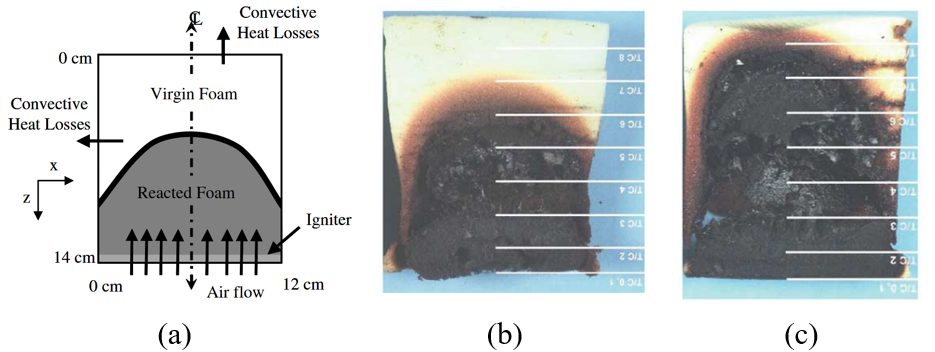
\includegraphics[width=1\textwidth]{Smoldering_experiment_presentation.png}
\caption{(a) Schematic representation of the experimental setup \cite{dodd_numerical_2009}. (b) and (c) images of the polyurethane foam sample after the experiment \cite{bar-ilan_forced_2004}.}
\label{fig:setup}
\end{figure}

\subsection{Numerical Model}

The experiment is simulated using \textsc{Gpyro} with gas transport solvers activated and by modeling the oxidation. The simulation is performed in one dimension. A time step of $\Delta t = 0.2$~s is used, together with a spatial grid resolution of 0.25~mm. Numerical convergence has been verified with respect to both the time step and the spatial resolution.

\paragraph{Chemical kinetics:}
The smoldering process is modeled using a seven-step kinetic mechanism \cite{dodd_numerical_2009}. Solid species are denoted by the subscript $(s)$ and gaseous species by $(g)$. The reactions are written using solid-phase stoichiometric coefficients $\theta_i$ and oxygen coefficients $\theta_{i,\mathrm{O_2}}$:

\begin{align}
\text{foam (s)} &\rightarrow \theta_1\,\text{\(\beta\)-foam (s)} + (1-\theta_1)\,\text{T-pyrolysate (g)} \label{eq:r1} \\
\text{\(\beta\)-foam (s)} &\rightarrow \theta_2\,\text{T-char (s)} + (1-\theta_2)\,\text{T-pyrolysate (g)} \label{eq:r2} \\
\text{T-char (s)} &\rightarrow \text{T-pyrolysate (g)} \label{eq:r3} \\
\text{foam (s)} + \theta_{4,\mathrm{O_2}}\,\mathrm{O_2} 
&\rightarrow \theta_4\,\text{char (s)} + (1-\theta_4+\theta_{4,\mathrm{O_2}})\,\mathrm{O_2} \text{-pyrolysate (g)} \label{eq:r4} \\
\text{\(\beta\)-foam (s)} + \theta_{5,\mathrm{O_2}}\,\mathrm{O_2} 
&\rightarrow \theta_5\,\text{char (s)} + (1-\theta_5+\theta_{5,\mathrm{O_2}})\,\mathrm{O_2} \text{-pyrolysate (g)} \label{eq:r5} \\
\text{char (s)} + \theta_{6,\mathrm{O_2}}\,\mathrm{O_2} 
&\rightarrow \theta_6\,\text{\(\alpha\)-char (s)} + (1-\theta_6+\theta_{6,\mathrm{O_2}})\,\mathrm{O_2} \text{-pyrolysate (g)} \label{eq:r6} \\
\text{\(\alpha\)-char (s)} &\rightarrow \text{products (g)} \label{eq:r7}
\end{align}



\paragraph{Kinetic parameters:}

The Arrhenius parameters associated with reactions~(\ref{eq:r1})--(\ref{eq:r7}) are summarized in Table~\ref{tab:kinetics smoldering}. The Arrhenius pre-exponential factor is denoted by $Z$, the activation energy by $E$, the reaction order by $n$, and the oxygen reaction order by $n_{\mathrm{O_2}}$. The reaction enthalpy is denoted by $\Delta H$. The table also reports the solid stoichiometric coefficients $\theta_i$ and the oxygen coefficients $\theta_{i,\mathrm{O_2}}$.

\begin{table}[H]
\centering
\caption{Kinetic parameters for the polyurethane foam smoldering reactions.}
\label{tab:kinetics smoldering}
\begin{tabular}{c c c c c c c c}
\toprule
Reaction & $Z$ (s$^{-1}$) & $E$ (kJ\,mol$^{-1}$) & $n$ & $n_{\mathrm{O_2}}$ & $\theta$ & $\theta_{\mathrm{O_2}}$ & $\Delta H$ (J\,kg$^{-1}$) \\
\midrule
\eqref{eq:r1} & $3.16\times10^{18}$ & 227.0 & 0.80 & 0 & 0.68 & 0.0 & $4.0\times10^{4}$ \\
\eqref{eq:r2} & $1.29\times10^{10}$ & 146.5 & 1.25 & 0 & 0.061 & 0.0 & $7.5\times10^{5}$ \\
\eqref{eq:r3} & $8.24\times10^{8}$  & 173.3 & 0.92 & 0 & 0.0 & 0.0 & $-2.5\times10^{6}$ \\
\eqref{eq:r4} & $1.37\times10^{15}$ & 188.0 & 0.48 & 1 & 0.38 & 0.186 & $-1.5\times10^{6}$ \\
\eqref{eq:r5} & $1.00\times10^{16}$ & 200.0 & 0.52 & 1 & 0.56 & 0.176 & $-1.6\times10^{6}$ \\
\eqref{eq:r6} & $1.00\times10^{15}$ & 201.0 & 1.30 & 1 & 0.24 & 1.14 & $-2.5\times10^{6}$ \\
\eqref{eq:r7} & $4.25\times10^{8}$  & 153.0 & 1.61 & 1 & 0.0 & 1.5 & $-2.5\times10^{6}$ \\
\bottomrule
\end{tabular}
\end{table}

\paragraph{Condensed-phase properties:}

The condensed-phase properties are reported in Table~\ref{tab:solid properties smoldering}. The temperature-dependent effective thermal conductivity is defined as $k_{\mathrm{eff}} = k_0 (T/T_{\mathrm{ref}})^{n_k} + \gamma \sigma T^3$, where $\gamma$ represents the pore radiation contribution and $\sigma$ is the Stefan--Boltzmann constant. The quantities $\rho$ and $\rho_s$ denote the bulk density and the skeleton density, respectively. The heat capacity is defined as $c_p = c_0 (T/T_{\mathrm{ref}})^{n_c}$. The emissivity is denoted by $\epsilon$, and $K$ is the permeability.

\begin{table}[h]
\centering
\caption{Condensed-phase thermophysical properties.}
\label{tab:solid properties smoldering}
\begin{tabular}{l c c c c c c c c c}
\hline
Species 
& $k_0$ & $n_k$ & $\gamma$ & $\rho$ & $\rho_s$ & $c_0$ & $n_c$ & $\epsilon$ & $K$ \\
& W\,m$^{-1}$\,K$^{-1}$ & - & m & kg\,m$^{-3}$ & kg\,m$^{-3}$ & J\,kg$^{-1}$\,K$^{-1}$ & - & - & m$^{2}$ \\
\hline
Foam & 0.05 & 1.6 & 0.001 & 26.5 & 900 & 1760 & 0.7 & 1.0 & $5.2\times10^{-9}$ \\
$\beta$-foam & 0.05 & 1.6 & 0.001 & 18.0 & 900 & 1760 & 0.7 & 1.0 & $1\times10^{-8}$ \\
T-char & 0.05 & 1.6 & 0.001 & 1.1 & 900 & 1760 & 0.7 & 1.0 & $3\times10^{-8}$ \\
Char & 0.05 & 1.6 & 0.001 & 10.0 & 900 & 1760 & 0.7 & 1.0 & $3\times10^{-8}$ \\
$\alpha$-char & 0.05 & 1.6 & 0.001 & 2.4 & 900 & 1760 & 0.7 & 1.0 & $3\times10^{-8}$ \\
\hline
\end{tabular}
\end{table}

\paragraph{Gas-phase properties:}

The gas-phase heat capacity is assumed constant, with $c_{p,g}=1100$~J\,kg$^{-1}$\,K$^{-1}$. Molecular weights noted $M$ and Lennard--Jones parameters used for diffusivity estimation are listed in Table~\ref{tab:gas properties smoldering}.

\begin{table}[h]
\centering
\caption{Gas-phase thermophysical properties.}
\label{tab:gas properties smoldering}
\begin{tabular}{l c c c}
\hline
Species & $M$ (g\,mol$^{-1}$) & $\sigma$ (\AA) & $\epsilon/k$ (K) \\
\hline
$\mathrm{O_2}$ & 32 & 3.434 & 113 \\
$\mathrm{N_2}$  & 28 & 3.667 & 99.8 \\
T-pyrolysate & 44 & 3.996 & 190 \\
$\mathrm{O_2}$-pyrolysate & 44 & 3.996 & 190 \\
Product & 44 & 3.996 & 190 \\
\hline
\end{tabular}
\end{table}

\paragraph{Boundary conditions:}

At the bottom boundary ($z=L$), the experimentally measured igniter temperature is imposed as a thermal boundary condition. At the top boundary ($z=0$), heat losses are modeled using a convective heat transfer coefficient of 10~W\,m$^{-2}$\,K$^{-1}$ combined with surface reradiation. Additionally, as the simulation is one-dimensional, radial heat losses are accounted for using a volumetric heat loss coefficient of 25~W\,m$^{-3}$\,K$^{-1}$.

For the pressure solver, a mass flux of 5.8~kg\,m$^{-2}$\,s$^{-1}$ is imposed at the inlet ($z=L$), corresponding to an air velocity of 5~mm\,s$^{-1}$ and an air density of 1.2~kg\,m$^{-3}$. Atmospheric pressure (1~bar) is imposed at the outlet.

For gas species, inlet mass fractions are fixed to $Y_{\mathrm{O_2}}=0.23$ and $Y_{\mathrm{N_2}}=0.77$.At the outlet, the flow is assumed to be dominated by advection (high Peclet number), and a free-outlet condition is imposed, where the concentration gradient is negligible and the gas exits freely:
\begin{equation}
\frac{\partial Y_j}{\partial z} = 0
\end{equation}

\subsection{Results}

\paragraph{Temperature evolution.}
Figure~\ref{fig:temperature} compares the predicted temperature histories at different axial locations with the experimental thermocouple measurements. The numerical results reproduce the main features of the experiment, including the arrival time of the thermal front and the order of magnitude of the peak temperatures. Overall, the agreement indicates that the thermal response of the foam is captured satisfactorily.

\begin{figure}[H]
\centering
\includegraphics[width=1\textwidth]{Thermocouple_Smoldering.png}
\caption{Comparison between predicted and measured temperature histories at different axial positions.}
\label{fig:temperature}
\end{figure}

\paragraph{Solid-phase composition.}
The evolution of the solid-phase composition is shown in Figure~\ref{fig:solid_composition} at four representative times: $t=400$~s, corresponding to the early stage of degradation; $t=600$~s and $t=800$~s, during active smolder propagation; and $t=1000$~s, near the end of the process. Degradation initiates with the formation of $\beta$-foam, which result from purely pyrolytic reactions (reaction ~\ref{eq:r1}). Slightly downstream, a second reaction zone develops, associated with oxidation reactions and the formation of char (reaction ~\ref{eq:r4} and ~\ref{eq:r5}). After the passage of these fronts, the remaining solid residue is mainly composed of $\alpha$-char and T-char, indicating that the smoldering reactions have largely completed.

\begin{figure}[H]
  \centering
  \begin{minipage}{0.48\linewidth}
    \centering
    \includegraphics[width=\linewidth]{Smoldering_sample_composition_t_400.png}\\
    \vspace{0.3em}
    \small \(t=400\) s
  \end{minipage}\hfill
  \begin{minipage}{0.48\linewidth}
    \centering
    \includegraphics[width=\linewidth]{Smoldering_sample_composition_t_600.png}\\
    \vspace{0.3em}
    \small \(t=600\) s
  \end{minipage}\\[0.8em]
  \begin{minipage}{0.48\linewidth}
    \centering
    \includegraphics[width=\linewidth]{Smoldering_sample_composition_t_800.png}\\
    \vspace{0.3em}
    \small \(t=800\) s
  \end{minipage}\hfill
  \begin{minipage}{0.48\linewidth}
    \centering
    \includegraphics[width=\linewidth]{Smoldering_sample_composition_t_1000.png}\\
    \vspace{0.3em}
    \small \(t=1000\) s
  \end{minipage}
  \caption{Solid-phase composition at $t=400$, 600, 800, and 1000~s.}
  \label{fig:solid_composition}
\end{figure}


\paragraph{Gas-phase composition inside the sample.}
Figure~\ref{fig:gas_composition} presents the gas-phase mass fractions inside the foam at the same four times. At $t=600$~s and $t=800$~s, oxygen is almost completely consumed within the smoldering front, as indicated by the oxygen mass fraction dropping to zero downstream of the reaction zone. This observation suggests that the thickness of the smoldering front is strongly controlled by the oxygen supply, with larger inlet fluxes expected to sustain wider reaction zones. Downstream of the front, the gas mixture is dominated by gaseous products of pyrolysis and oxidation. At $t=1000$~s, once degradation has ceased, the remaining pyrolysis gases  exit the sample, and the gas composition is that of the injected air.

\begin{figure}[H]
  \centering
  \begin{minipage}{0.48\linewidth}
    \centering
    \includegraphics[width=\linewidth]{Smoldering_gas_mass_fraction_t_400.png}\\
    \vspace{0.3em}
    \small \(t=400\) s
  \end{minipage}\hfill
  \begin{minipage}{0.48\linewidth}
    \centering
    \includegraphics[width=\linewidth]{Smoldering_gas_mass_fraction_t_600.png}\\
    \vspace{0.3em}
    \small \(t=600\) s
  \end{minipage}\\[0.8em]
  \begin{minipage}{0.48\linewidth}
    \centering
    \includegraphics[width=\linewidth]{Smoldering_gas_mass_fraction_t_800.png}\\
    \vspace{0.3em}
    \small \(t=800\) s
  \end{minipage}\hfill
  \begin{minipage}{0.48\linewidth}
    \centering
    \includegraphics[width=\linewidth]{Smoldering_gas_mass_fraction_t_1000.png}\\
    \vspace{0.3em}
    \small \(t=1000\) s
  \end{minipage}
  \caption{Gas-phase mass fractions inside the sample at $t=400$, 600, 800, and 1000~s.}
\label{fig:gas_composition}
\end{figure}


\paragraph{Smolder front propagation.}
Figure~\ref{fig:smolder_front} focuses on the char mass fraction, which is a direct product of oxidation reactions (see reactions~\ref{eq:r4}--\ref{eq:r5}). Regions with non-zero char mass fraction clearly identify the active smoldering zone. The displacement of the char peak over time reveals a steady propagation of the smolder front along the sample. The propagation velocity is estimated by tracking the position of this peak, yielding a value of approximately 0.25~mm\,s$^{-1}$. This value is consistent with experimentally reported measurements \cite{bar-ilan_forced_2004}, supporting the validity of the numerical model.

\begin{figure}[H]
\centering
\includegraphics[width=0.75\textwidth]{Smoldering_front_propagation.png}
\caption{Smolder front propagation inferred from the spatial distribution of char mass fraction.}
\label{fig:smolder_front}
\end{figure}


\paragraph{Gas mass fluxes.}
Figure~\ref{fig:mlr} shows the net mass flux of gaseous species, defined as the difference between the outlet and inlet mass flow rates. The oxygen mass flux is negative, indicating oxygen consumption due to oxidation reactions occurring within the smoldering front. Although nitrogen is inert and does not participate in any reaction, a non-zero nitrogen mass flux is observed. This behavior is attributed to gas expansion caused by the temperature rise during degradation, which induces an outward flow of nitrogen driven by density variations.

\begin{figure}[H]
\centering
\includegraphics[width=0.75\textwidth]{MLR_Smoldering.png}
\caption{Net gaseous mass fluxes during the smoldering process.}
\label{fig:mlr}
\end{figure}


\ifdefined\standalone
\bibliographystyle{unsrt}
\bibliography{smoldering}
\end{document}
\fi






